\documentclass[a4paper, 11pt, oneside]{article}
\usepackage{minted}
\usepackage[utf8]{inputenc}
\usepackage[T1]{fontenc} 
\usepackage{fouriernc}
\usepackage{listings} 
\lstset{language=C}   
\usepackage{xcolor}
\usepackage{float}

\usepackage{tabularx}
\usepackage{amsmath}  
\usepackage{graphicx}
\usepackage[margin=1in,letterpaper]{geometry}
\usepackage{cite} 
\usepackage[final]{hyperref} 
\hypersetup{
	colorlinks=true,       % false: boxed links; true: colored links
	linkcolor=blue,        % color of internal links
	citecolor=blue,        % color of links to bibliography
	filecolor=magenta,     % color of file links
	urlcolor=blue         
}
\usepackage{blindtext}

\begin{document} 
\begin{titlepage} 
\centering
\scshape
\vspace*{\baselineskip}
\rule{\textwidth}{1.6pt}\vspace*{-\baselineskip}\vspace*{2pt} 
\rule{\textwidth}{0.4pt} 
\vspace{0.75\baselineskip} 

{\LARGE Run and Shoot}

\vspace{0.75\baselineskip} 
\rule{\textwidth}{0.4pt}\vspace*{-\baselineskip}\vspace{3.2pt}
\rule{\textwidth}{1.6pt}
\vspace{2\baselineskip}

	Software Design \& Project Set-up (Deliverable 2) % Subtitle or further description
	
	\vspace*{3\baselineskip} % Whitespace under the subtitle
	
	%------------------------------------------------
	%	Editor(s)
	%------------------------------------------------
	
	Students:
	
	\vspace{0.5\baselineskip} % Whitespace before the editors
	
	{\scshape\Large El-Habrouk Jaser \\ Firoozishahmirzadi Parichehreh \\ Layeghi Mahsa \\ Xu Jin} 
	
	\vspace{3\baselineskip} 
	
	%\textit{Carleton University} % Editor affiliation
	
		
	Course Instructor:
	
	\vspace{0.5\baselineskip} % Whitespace 
	
	{\scshape\Large Cristina Ruiz Martin}
	
	\vspace{3\baselineskip} % Whitespace 
	
	Course Title:
	\vspace{0.5\baselineskip} % Whitespace 
	
	{\scshape\Large Software Development with C} 
	
	\vfill % Whitespace between editor names and publisher logo
	
	
	\vspace{0.3\baselineskip} % Whitespace under the publisher logo
	
	Tuesday, 20\textsuperscript{th} of October, 2020 % Publication year
\end{titlepage}

\section{Menu flowchart and explanation~\ref{fig:menu}}
\begin{figure}
    \centering 
    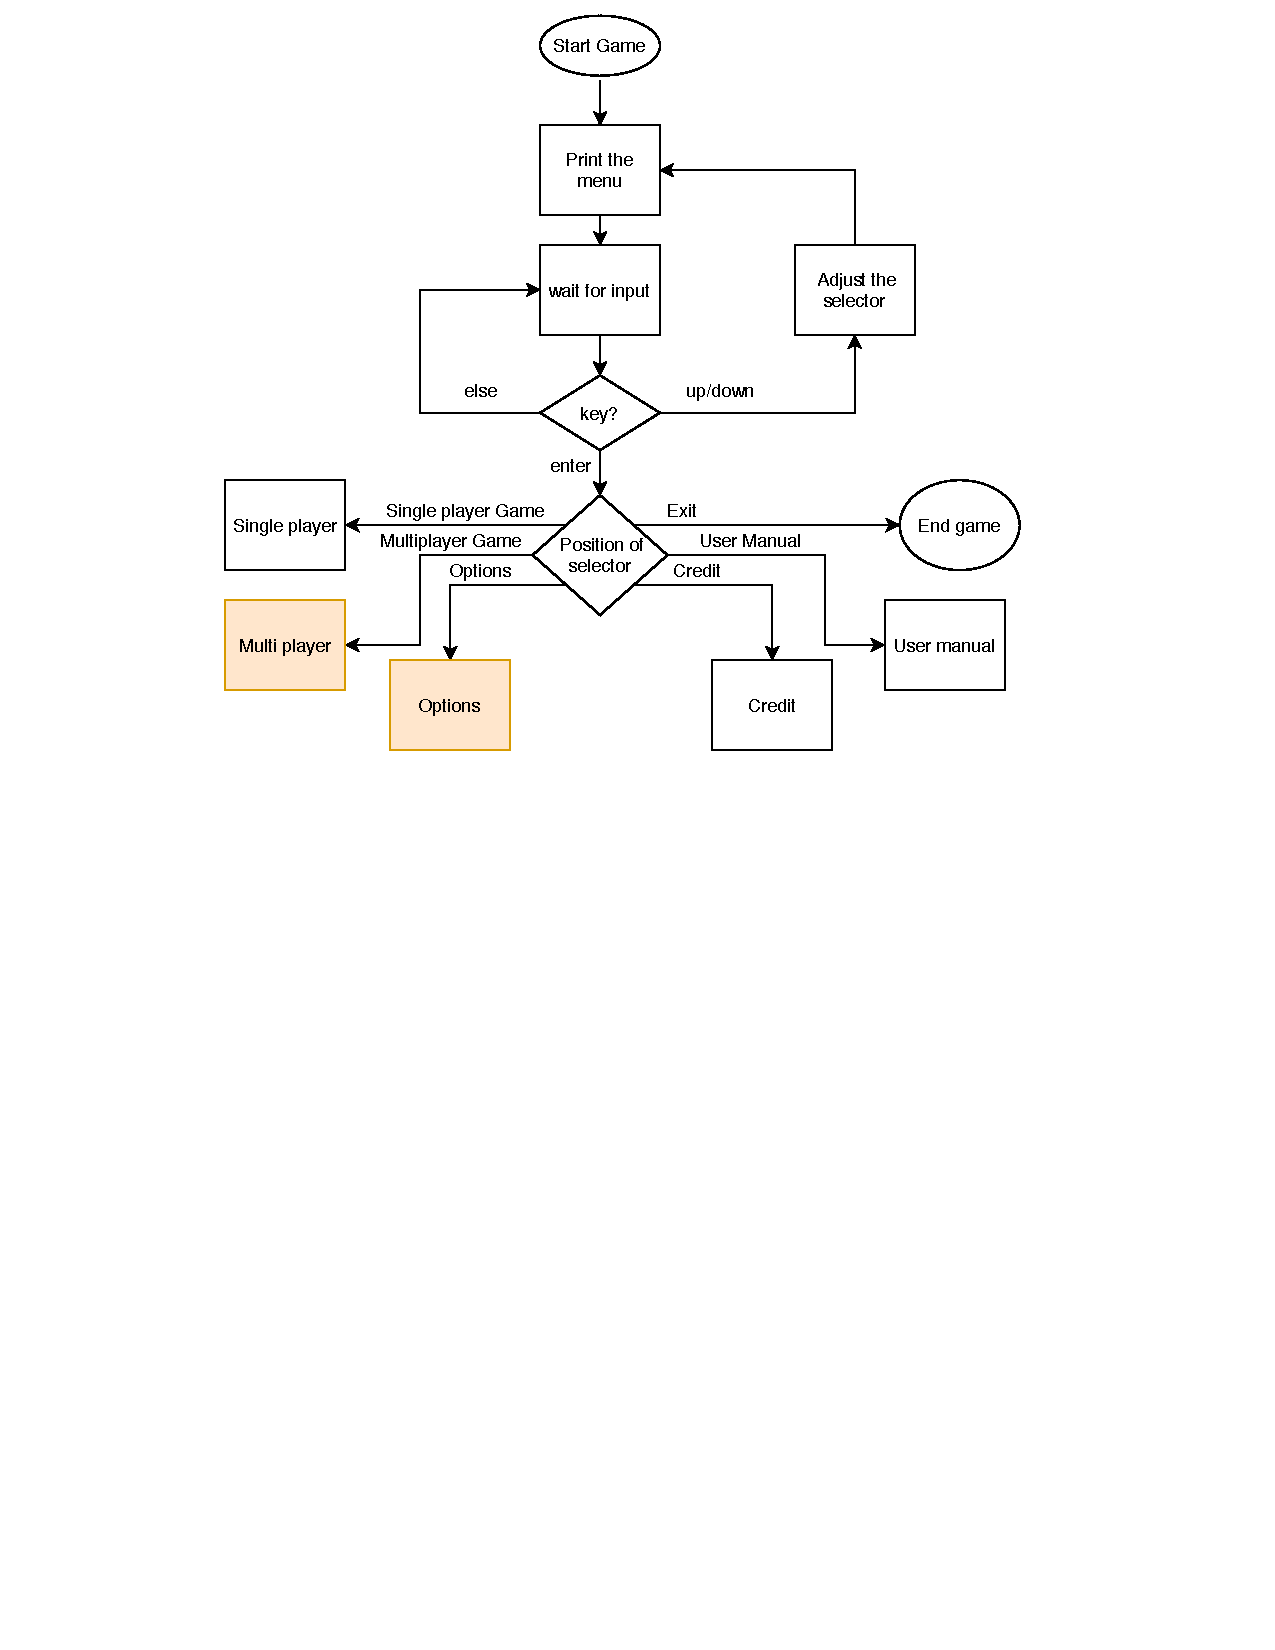
\includegraphics[width=0.8\columnwidth]{menu.pdf}
    \caption{Menu flowchart. white blocks are implemented in first release and \textcolor{orange}{orange} blocks are implemented in second release. }
    \label{fig:menu}
\end{figure}

This section explains the flow of our program since execution starts until it finishes. 
As it is shown in Figure \ref{fig:menu}, initially, we print a menu for the game. There are multiple choices on the game menu and user can go through each of them and press enter to select one. So, program is waiting for the user to press a key.
There is a selector which places besides each menu item. The user can see the selector and be informed on its selection. Adjust the selector block is responsible for this operation.
Next step decides what to do based on the user's choice. 
As we seen in Figure~\ref{fig:menu}, we may go on six different scenarios: user manual, single player, multiplayer, options, credit and end game which will be explained in detail in the coming sections.

\subsection{Menu functions prototype}
In this section we define the required functions prototypes and its relation to flow chart. Comments above each function mention the associated block, the release, and assignee.

\begin{minted}{c}
#define MAX_ITEM_SIZE 100
#define NUM_OF_ITEMS 6

typedef enum {
	USER_MANUAL,
	SINGLE_PLAYER,
	MULTI_PLAYER,
	OPTION,
	CREDIT,
	EXIT,	
} MenuSelector;

typedef struct MenuItem {
	char str[MAX_ITEM_SIZE];
} MenuItem;

typedef struct Menu {
	MenuSelector selector;
	MenuItem items[NUM_OF_ITEMS];
} Menu;

/* Block: Print the menu - first release
 * Assigned to: Jaser
 * Prints the game start up menu on the consol.
 * Input: menu
 * Return: void */
void printMenu(Menu menu);

/* Block: Adjust the selector - first release
 * Assigned to: Jaser
 * Updates the selector position according to input key.
 * Input: menu_p, arrowKey
 * Output: menu_p
 * Return: void */
void updateSelector(Menu* menu_p, int arrowKey);

/* Block: Options - second release
 * Assigned to: Jaser
 * Calls functions related to options
 * Input: void
 * Output: void
 * Return: void*/
void option(void);

/* Block: Single player - first release
 * Assigned to: Pari
 * Calls functions related to Single Player Setup 
 * on Level 2 flowchart
 * Input: void 
 * Output: void
 * Return: void */
void singlePlayer(void);

/* Block: Credit - first release
 * Assigned to: Mahsa
 * shows information about the credit.
 * Input: void 
 * Output: void
 * Return: void */
void credit(void);

/* Block: Multi player - second release
 * Assigned to: Jin
 * Calls functions related to multiplayer setup.
 * Input: void 
 * Output: void
 * Return: void */
void multiPlayer(void);

/* Block: End game - first release
 * Assigned to: Mahsa
 * Exit from the game
 * Input: void 
 * Output: void
 * Return: void */
void exit(void);

/* Block: User manual - first release
 * Assigned to: Jin
 * displays a user manual for the player (how to Play).
 * Input: void 
 * Output: void
 * Return: void */
void userManual(void);
\end{minted}
\section{Single player flowchart and explanation~\ref{fig:singleplayer}}

\begin{figure}
    \centering 
    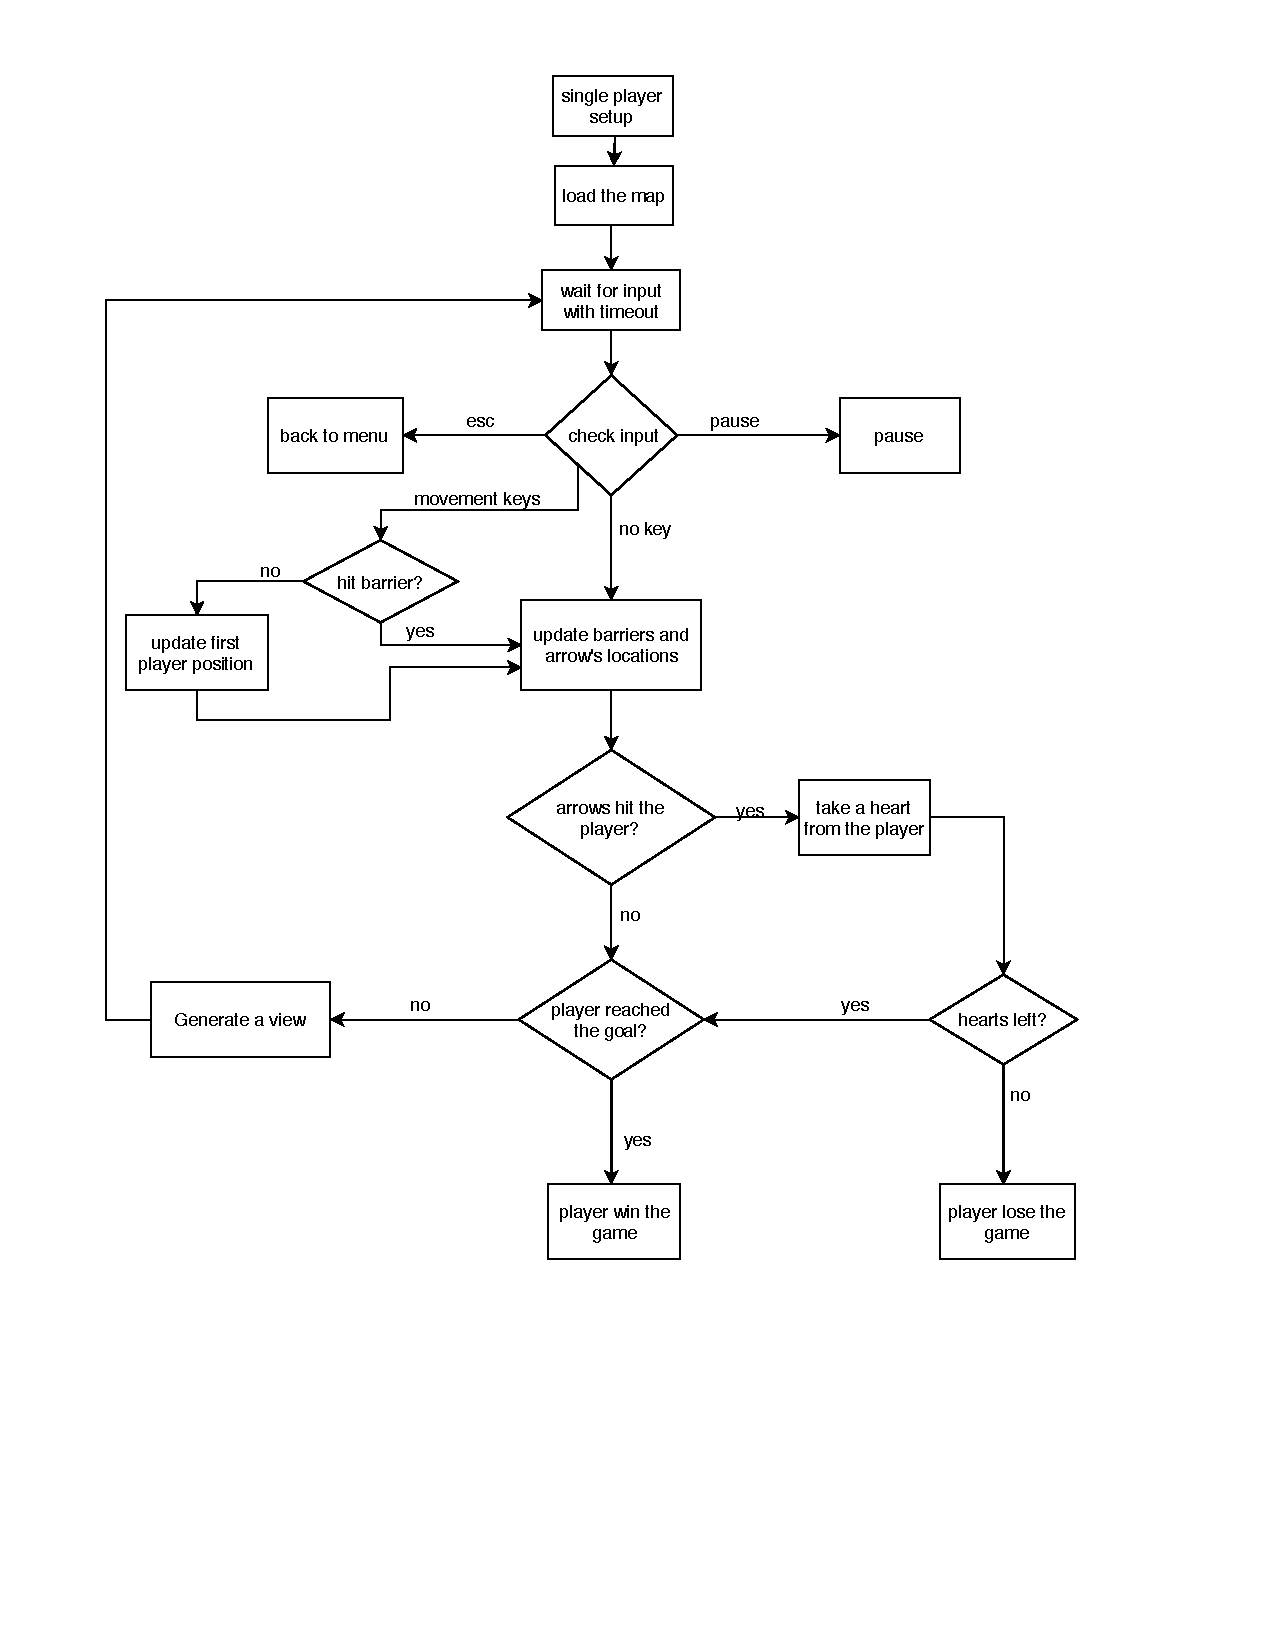
\includegraphics[width=\columnwidth]{singleplayer.pdf}
    \caption{Single player block flowchart. white blocks will be implemented in the first release.}
    \label{fig:singleplayer}
\end{figure}

This flow chart explains all the steps happening on single player mode. 
As it is shown in Figure~\ref{fig:singleplayer}, load the map block reads the map from a text file. Next, we do some setups for single player game based on the map. In these setups we define a map with position of the player, the goal, the barriers and the arrows.
We should then read the input keyboard buffer and wait for input. The reading process is done within a limited time and there exist a timeout which expires if no input is provided within that time. Then the program checks the input to see what key has entered. If pause button is entered, program goes to pause game state. If escape button is pressed, program goes to menu. If no keys has entered, program updates the position of barriers and arrows as they are moving objects. If entered keys are movement keys, program first check if the player's move is permitted or not (checks map walls and barriers); if yes, then program updates the player position, barriers and arrows locations, and checks if the player is hit. If player can not move, program only updates barriers and arrows and does not change player's location. If player is hit by an arrow, it loses one heart and immediately checks if there is any heart left for the player. If the player loses all of its hearts, player loses the game. If the player has still a heart, program check if the player reaches the goal. Player wins the game if it reach the goal, otherwise program \textcolor{blue}{\bf generate a view} to display any updates on the map. Then wait for input key and it will continue until the player wins or loses the game.
If there exist any graphic related procedures it is done in generate view process, and logic of the game does not need to worry about graphics.

\subsection{Single player functions prototypes}
In this section we define the required functions prototypes and its relation to flow chart~\ref{fig:singleplayer}. We define some functions and the rest of the code will be in a main function. Comments above each function mention the associated block, the release, and assignee.

\begin{minted}{c}
#define MAP_MAX_NUM_OF_BARRIERS 10
#define MAP_MAX_NUM_OF_ARROWS 20
#define MAX_NAME_SIZE 100

typedef struct Position {
	int x;
	int y;
} Position;

typedef enum {
	DIRECTION_RIGHT,
	DIRECTION_LEFT,
	DIRECTION_UP,
	DIRECTION_DOWN
} Direction;

typedef enum {
	SPEED_LOW,
	SPEED_NORMAL,
	SPEED_HIGH,
} Speed;

typedef struct MapSpace {
	int xMin;
	int xMax;
	int yMin;
	int yMax;
} MapSpace;

typedef struct MapBarrier {
	Position currentPos;
	int length;
	Direction currectDir;
} MapBarrier;

typedef struct MapArrow {
	Position currentPos;
	Speed speed;
} MapArrow;

typedef struct Player {
    char name[MAX_NAME_SIZE];
	Position currentPos;
	int heart;
} Player;

typedef struct Goal {
	Position goal;
} Goal;

typedef struct Map {
	MapSpace space;
	int numberOfBarriers;
	int numberOfArrows;
	MapBarrier barrier[MAP_MAX_NUM_OF_BARRIERS];
	MapArrow arrow[MAP_MAX_NUM_OF_ARROWS];
	Goal goal;
	Player player;
} Map;

/* Block: Load the map - first release
 * Assigned to: Pari
 * Load map information from an input file using provided information
 * from options.
 * Input: file_p, mapSelector
 * Output: Map */
Map loadMap(FILE* file_p, int mapSelector);

/* Block: Update barriers and arrow's locations - first release
 * Assigned to: Jin
 * Update barrier position in the map
 * Input: barrier, space
 * Output: barrier 
 * Return: void */
void updateBarrier(MapBarrier* barrier, MapSpace space);

/* Block: Update barriers and arrow's locations - first release
 * Assigned to: Jaser
 * Update arrows' position in the map
 * Input: arrow, space
 * Output: arrow
 * Return: void */
void updateArrow(MapArrow* arrow, MapSpace space);

/* Block: Pause - first release
 * Assigned to: Pari
 * It continues the game when the game is on pause 
 * Input: void
 * Return: void */
void continueGame(void);

/* Block: Pause - first release
 * Assigned to: Jin
 * It pause the game
 * Input: void
 * Return: void */
void pauseGame(void);

/* Block: Back to menu - first release
 * Assigned to: Jaser
 * It goes back to Menu
 * Input: void
 * Return: void */
void backToMenu(void);

/* Block: Hit barrier? - first release
 * Assigned to: Mahsa
 * Check if there is any barrier on the way of player.
 * Input: player, barrier
 * Output: 0 ---> player no hit & 1---> player is hit
 * Return: int */
int isBarrierHit(Player player, MapBarrier* barrier_p, MapSpace space);

/* Block: Update player position - first release
 * Assigned to: Mahsa
 * Update player position in the map.
 * Input: player, arrowKey
 * Output: player 
 * Return: void */
void updatePlayerPos(Player* player_p, int arrowKey);

/* Block: Arrows hit the player - first release
 * Assigned to: Pari
 * check if the player is hit by arrows.
 * Input: player, arrow
 * Output: 1 ---> if the player is hit
 * Return: int */
int isPlayerHit(Player player, MapArrow* arrow_p);


/* Block: Takes a heart from the player - first release
 * Assigned to: Jin
 * Takes a heart from the player.
 * Input: player
 * Output: player
 * Return: void */
void takeHeart(Player* player_p);

/* Block: hearts left - first release
 * Assigned to: Jaser
 * Check if the player lost all its heart.
 * Input: player
 * Output: 1 ---> if the player lost all its heart
 * Return: int */
int isGameOver(Player player);

/* Block: player lose the game - first release
 * Assigned to: Pari
 * inform player that he/she lost the game
 * Input: player
 * Output: void
 * Return: void*/
void gameOver(Player player);


/* Block: player reached the goal - first release
 * Assigned to: Jaser
 * Checks if the player reached the goal
 * Input: player, goal
 * Output: 1 ---> if the player reached the goal
 * Return: int */
int isReachGoal(Player player, Goal goal);

/* Block: player win the game - first release
 * Assigned to: Mahsa
 * inform player that he/she win the game
 * Input: player
 * Output: void
 * Return: void*/
void winGame(Player player);

/* Block: generate a view- first release
 * Assigned to: Jin
 * Generate a 2d graphic map using updated information
 * Input: map
 * Return: void */
void updateView(Map map);

\end{minted}
\section{Multi-player flowchart and explanation~\ref{fig:multiplayer}}

\begin{figure}
    \centering 
    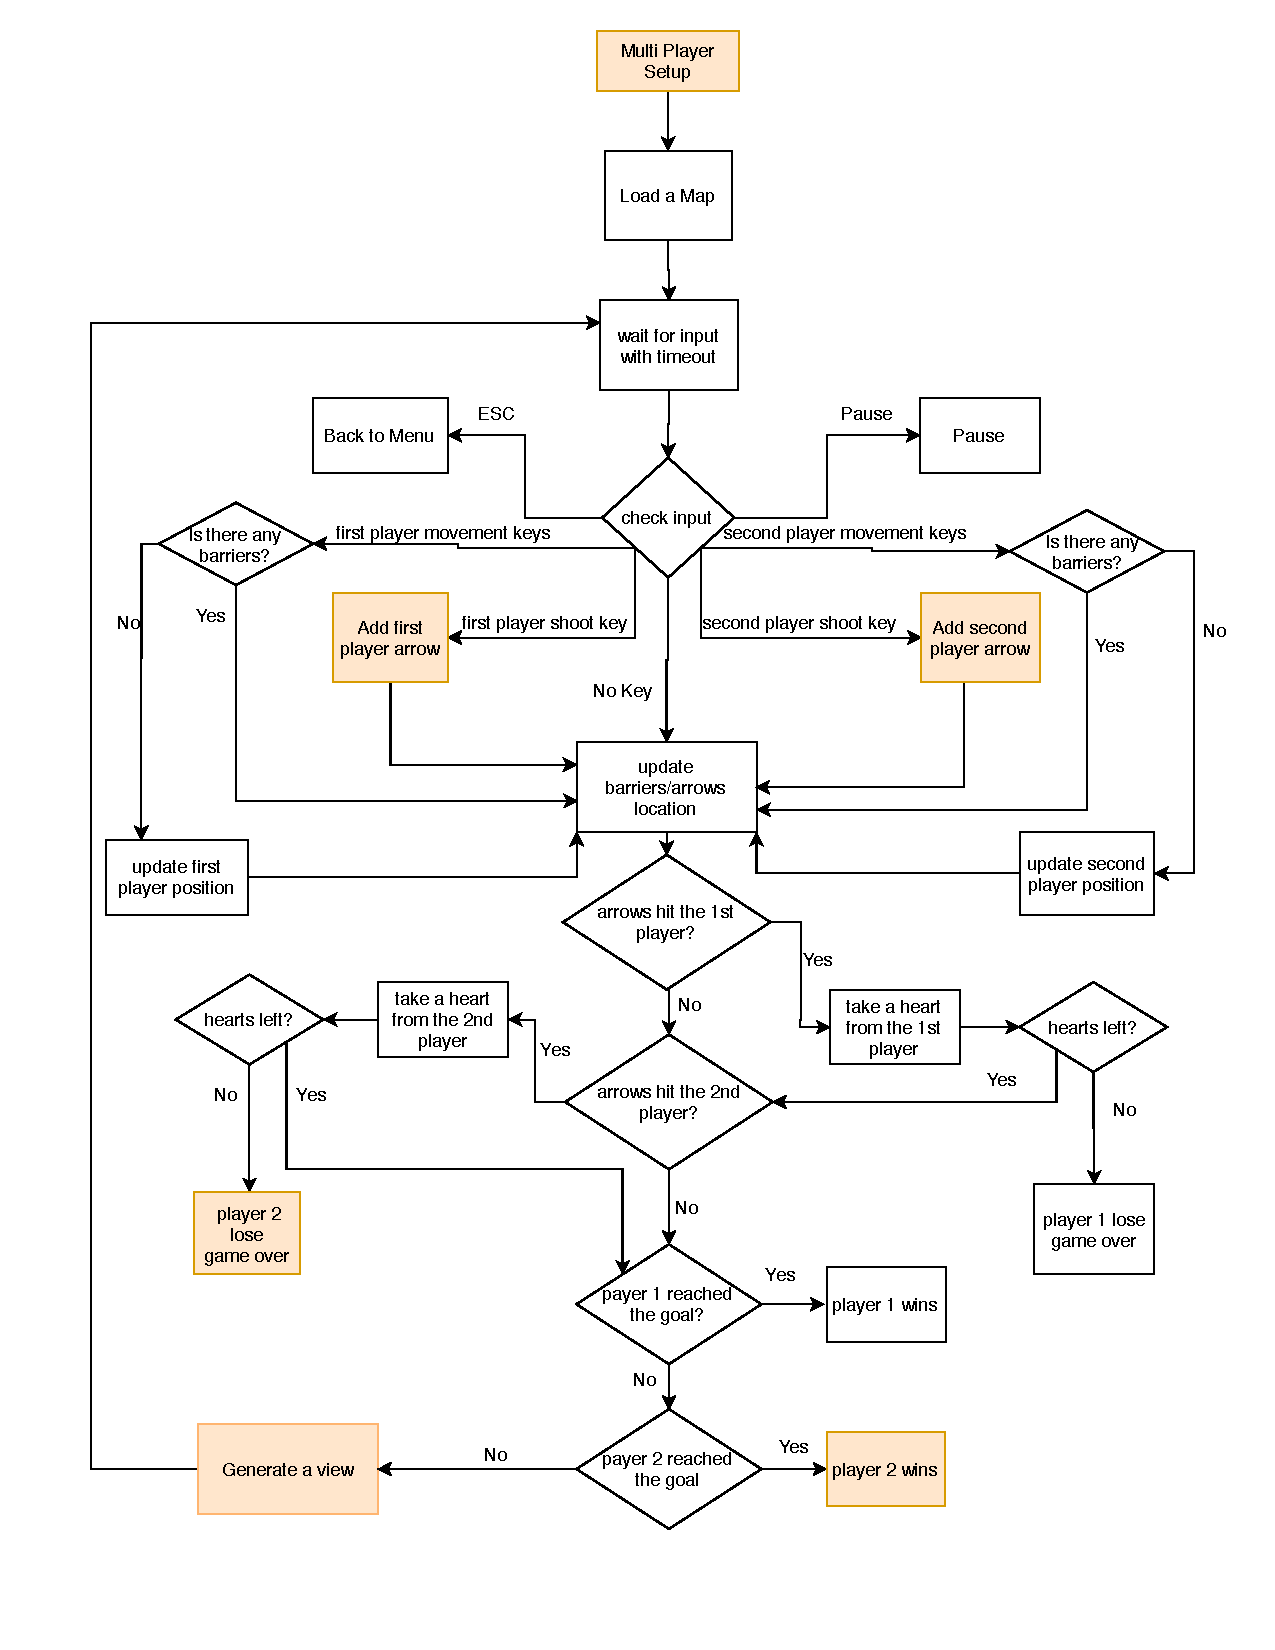
\includegraphics[width=0.9\columnwidth]{multiplayer.pdf}
    \caption{Multi-player block flowchart. Blocks which are in \textcolor{orange}{orange} will be implemented for the second release. Some functions and blocks are used in both single player and multi-player mode which are in white color.}
    \label{fig:multiplayer}
\end{figure}

This Flow chart explains all the steps happening on multi-player mode. 
As it is shown in Figure~\ref{fig:multiplayer}, after we select the multi-player option in Menu function, we begin from the load Map step, where we should read the map from a text file. 
Next, we do some setups for multi-player game based on the map. 
In these setups, we define a map with positions of two players, the goal, the barriers and the arrows. 
We should then get input from keyboard. 
We should check if there was any input given for either player. 
If not, we should update the position of barriers/arrows as they are moving objects. 
If either player hits delete/ backspace button, we go back to menu. 
If hits space button, we go to the state of pause game. 
If hits space button again, we should continue the game. 
In both continue and pause state, we go back to get input from keyboard and wait for either player to enter another key. 
Given the movement keys, we update the position of first/second player accordingly. 
Also, by giving the specific shoot keys, we then generate arrows from the position of the shooting player. 
Both players need to run in different directions controlled by movement keys to avoid being shot by moving arrows. 
The process of dealing with barriers, losing hearts and reaching the goal for each player is the same as single player mode. 
By continuing to check the remaining hearts of them during the whole movement, we can know which player loses the game earlier than the other, which is the same way as judging whether the game is over for single player mode. 
As for the win scenario, only if the player alive reaches the final goal. 
If not reaching the win state ever, the program will generate a view afterwards and continue to wait for another key input.

\subsection{Multi-player functions prototypes}

In this section we define the required functions prototypes and its relation to flow chart~\ref{fig:singleplayer}. We define some functions and the rest of the code will be in a main multi-player function. Comments above each function mention the associated block, the release, and assignee. Some functions are in common for both single player and multi-player mode.We did not mention then again as they already described.

\begin{minted}{c}
/**
 * @brief timer
 * @author Pari
 * First Release
 */
Uint32 timer_callback(Uint32, void*);

/**
* @brief generate_view_multi function
* @author Jin
* Release two
* This function is to generate a graphic map using updated information
* @param[in] p_window a SDL window which is passed from the main function.
* @param[in] p_map a defined map which is passed from the main function.
* @return: void
*/
void generate_view_multi(SDL_Window* p_window, map_t* p_map);

/**
 * @brief Generates a bullet
 * @author Mahsa
 * Release two
 * This function generates a bullet in the player's current position
 * and initialize the speed and direction.
 * @param[in] map represent the map structure which has players' position.
 * @param[in] player_num represent the player index: PLAYER_1/PLAYER_2.
 */
void shoot(map_t* map, player_index_t player_num);

/**
 * @brief updates the position of generated bullet
 * @author Mahsa 
 * Release two
 * This function shoot a bullet in a direction in which an oppenent exists.
 * @param [in] map represent the map structure which has bullet's position and direction.
 */
void update_bullet(map_t* map, player_index_t player_num);

/**
 * @brief Checks if a bullet hit a player.
 * @author Mahsa 
 * Release two
 * This function checks if the player is hit by oppent's bullet.
 * @param [in] map represent the map structure which has 
 * player position and bullets' positions.
 * @param [in] player_index  can be PLAYER1 or PLAYER2.
 * @return flag if the player is hit, flag = 1, otherwise flag = 0.
 */
int is_bullet_hit(map_t* map, player_index_t player_index);
\end{minted}
% \vspace{0.75\baselineskip} 
% \rule{\textwidth}{0.4pt}\vspace*{-\baselineskip}\vspace{3.2pt}
% \rule{\textwidth}{1.6pt}
% \vspace{2\baselineskip}
\section{Options flowchart and explanation~\ref{fig:options}}
\begin{figure}
    \centering 
    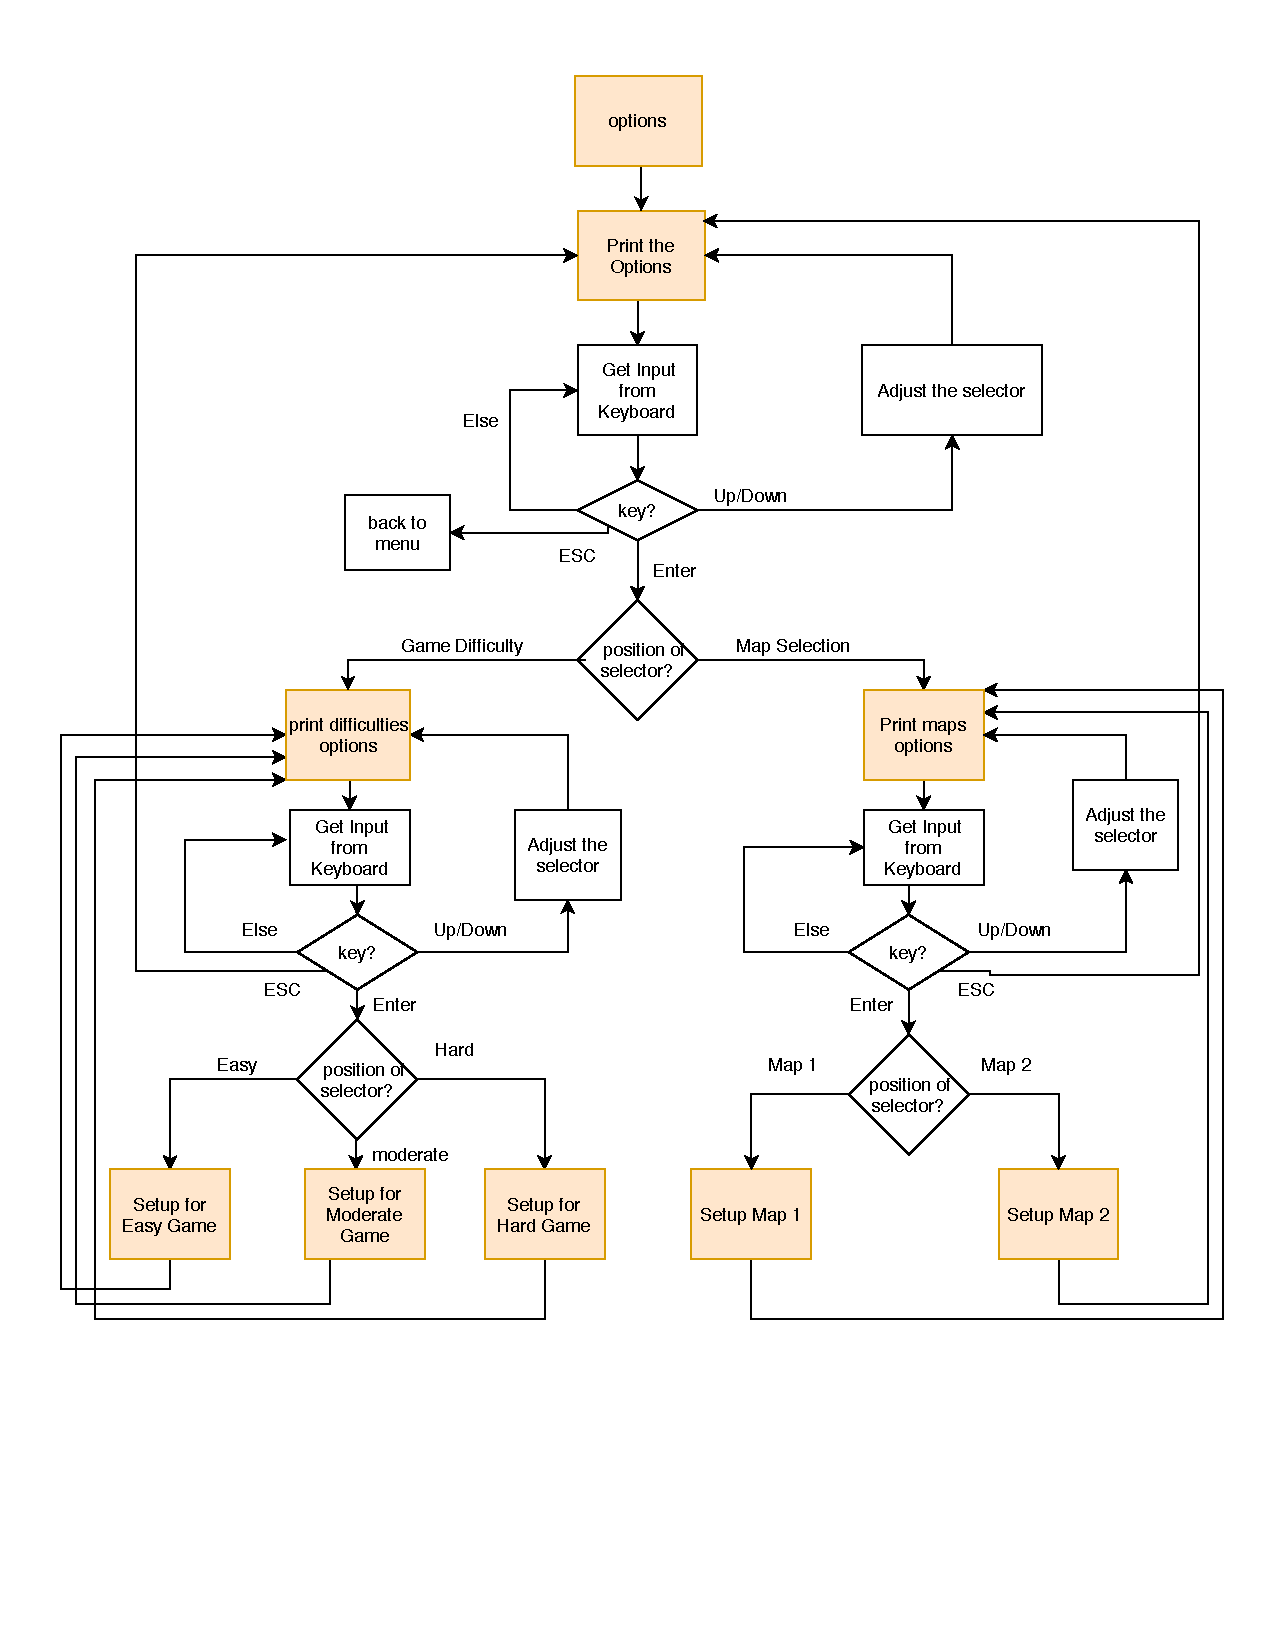
\includegraphics[width=\columnwidth]{options.pdf}
    \caption{Options block flowchart. Blocks which are in \textcolor{orange}{orange} will be implemented for the second release. Some functions and blocks are used in both menu and options which are in white color.}
    \label{fig:options}
\end{figure}

This flow chart explains all the steps happening on the options block. 
As it is shown in Figure~\ref{fig:options} initially, options items which are game difficulties are printed for the user. 
Next, according to the user input key the program goes to one of the following states: 
Enter key, Choose one difficulty level between easy, intermediate, and hard items and go back to menu.
Up/down key, go up and down between option's items.
The selected difficulty is used to do the single-player and multi-player setup later.

\subsection{Options functions prototypes}

In this section we define the required functions prototypes and its relation to flow chart~\ref{fig:options}.

\begin{minted}{c}
/**
 * @enum options_items_t
 * The enumeration of option items.
 */
typedef enum option_items{
    OPTION_ITEM_EASY,
    OPTION_ITEM_INTERMEDIATE,
    OPTION_ITEM_HARD,
    OPTION_ITEM_NUM_OF_ITEMS,
}option_items_t;

/**
 * @typedef option_t
 * A structure represents option's item.
 */
typedef struct option{
    option_items_t selector;
    item_t items[OPTION_ITEM_NUM_OF_ITEMS];
} option_t;

/**
* @brief Prints the game different difficulty options on an SDL window.
* @author Jaser
* Second release.
* @param[in] p_window A SDL window is passed to the function.
* @param[in] p_options A structure represents options item.
* @return void
*/
void print_options(SDL_Window* p_window, option_t* p_options);
\end{minted}

\end{document}